% In the optional argument of the frame below, i.e. \begin{frame}{Title \hfill logo \hfill UNCC Logo}, add a logo for your section in place of the "figs/topic3White.pdf".  Make sure it has a transparent background, and that it uses white elements to ensure it's visible.

\section{Click2ExAnimation}
\begin{frame}{Example Animation \hfill 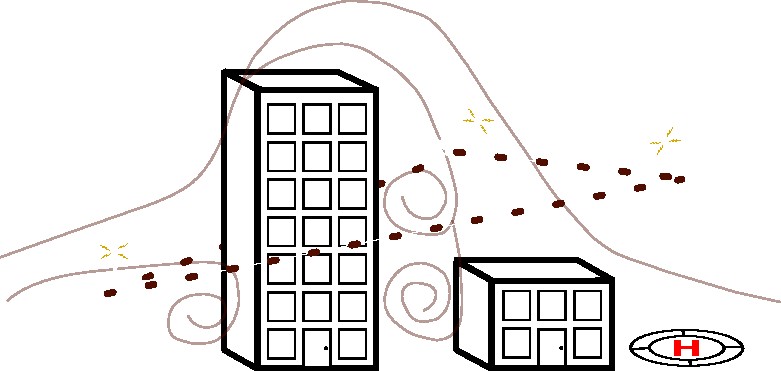
\includegraphics[height=.7cm]{figs/exTopicLogo.pdf} \;\;\;\;\; 
\includegraphics[height=.5cm]{figs/uncc/whiteUNCCLogo.eps}}
    These animations only really work when viewed in Adobe reader.  Adobe reader has a presentation mode, and during the presentation, you just use the controls under the animation frame to play the animation.

    \begin{columns}[T,onlytextwidth]
        \column{0.8\textwidth}
            \animategraphics[loop,controls,width=\linewidth]{70}{figs/gpAnimation/gpAnimationFrame-}{0}{85}
        \column{0.2\textwidth}
            \begin{align*}
                L &= 1.5 \text{ m} \\
                \sigma^{2} &= 4 \text{ m}^{2}\\
                \sigma_{n}^{2} &= 0.6 \; (\text{m/s})^{2} \\
                \mu_{w} &= -8 \text{ m/s}
            \end{align*}
    \end{columns}
\end{frame}
